\subsection{Drawer}\label{sec:launcher:drawer}
The drawer is a separate view that is situated in the left-hand side of the \textit{Home} activity.
Its main purpose is to allow \launcher users to apply a new colourscheme to their installed \giraf applications.

The concept of a drawer is a component that can be shown and hidden at will.
This means that only part of the drawer is visible at all time; it can be dragged towards the centre of the screen to reveal its contents.
Apart from enabling the users to switch colours of their installed \giraf apps, it also contains various informative widgets.
These widgets are a calendar, implemented as \lstinline{GWidgetCalendar}, a server connection indicator, implemented as \lstinline{GWidgetConnectivity}, and a logout button, implemented as \lstinline{GWidgetLogout}.
The implementations of these widgets are a part of \lstinline{GirafComponents}, a separate project in the \giraf system that handles customized User Interface components.
It should be utilized throughout all \giraf applications to make them look and feel the same.

Illustrations of the drawer in closed and opened positions can be seen in \cref{fig:drawerclosed,fig:draweropened} respectively.

\begin{figure}[h] % Billeder af draweren i åben og lukket tilstand
\centering
	\begin{subfigure}[b]{.48\textwidth}
	\centering
	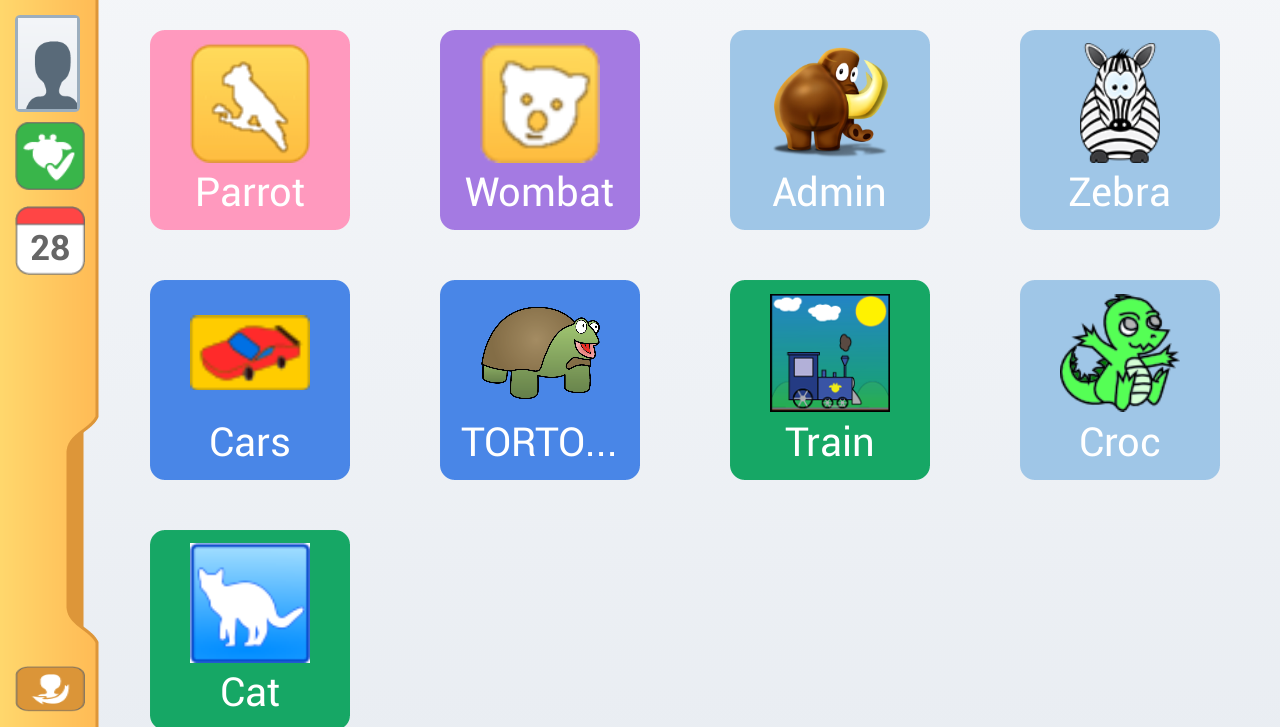
\includegraphics[width=\textwidth]{screenshots-old-giraf/giraf-homeactivity.png}
	\caption{Drawer closed.}
	\label{fig:drawerclosed}
	\end{subfigure}
	\hfill
	\begin{subfigure}[b]{.48\textwidth}
	\centering
	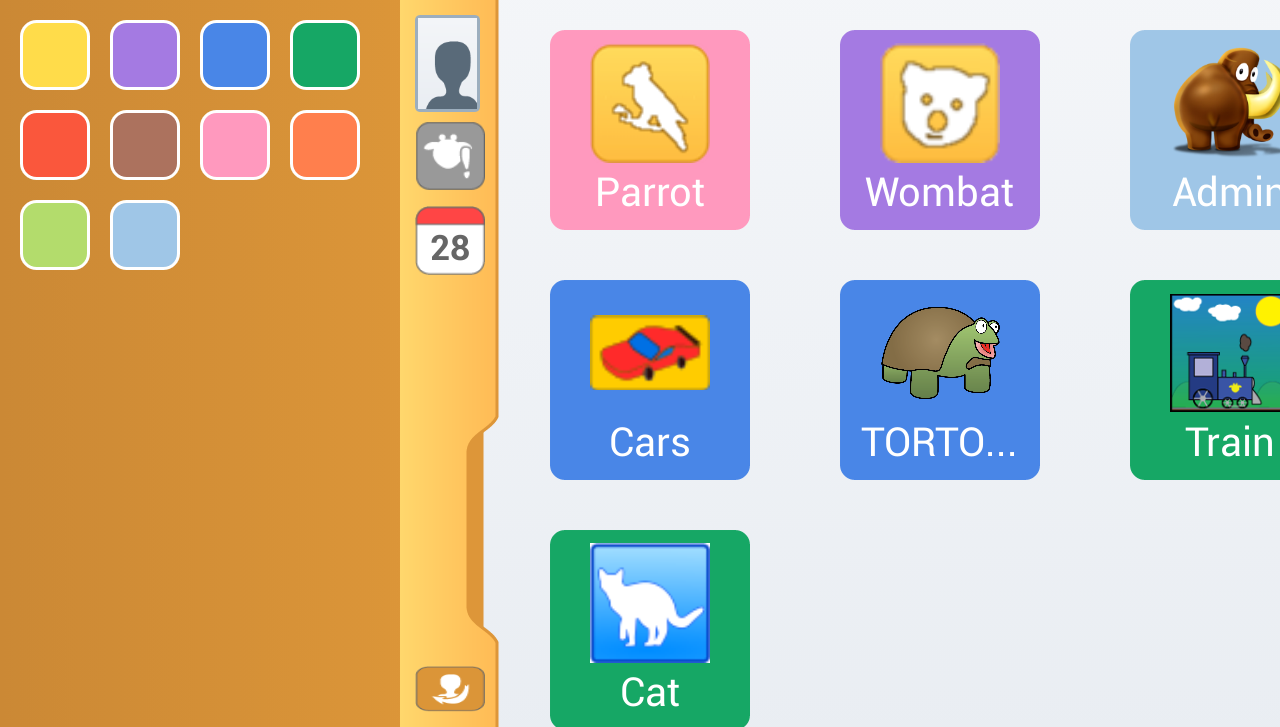
\includegraphics[width=\textwidth]{screenshots-old-giraf/giraf-drawer-fullyextended.png}
	\caption{Drawer fully extended.}
	\label{fig:draweropened}
	\end{subfigure}
\caption{States of the drawer component shown on \textit{Home} activity.}
\label{fig:drawerstates}
\end{figure}

While the drawer basically worked as intended, we identified a number of possibilities for making its use more fluent.
This section describes the original drawer, the desired improvements and the final result.

\subsubsection{The Original Drawer}

The original drawer would open by pressing and holding the bar and sliding it to the right.
While being opened, the drawer would push the application icons along with it to the right, resulting in some icons disappearing off-screen to the right.
Furthermore, the drawer would stop when pressure was released from the touchscreen, meaning it could be left in a half-open, half-closed state.
To change the colour of an application, a colour could be drag-and-dropped onto an icon. The result would be immediately apparent, as the colour framing the icon would change to the selected colour.

The code working this animation was based on an \lstinline{OnTouchListener}, focusing mainly on the \lstinline{MotionEvent.ACTION_MOVE} event.
\lstinline{MotionEvent.ACTION_MOVE} would set the position of the entire drawer, panel and bar, to the exact point it had currently been moved to and redraw the elements.
Because the \lstinline{ScrollView} containing the application icons was set to \lstinline{android:layout_toRightOf} in the layout XML files, the \lstinline{ScrollView} would adjust itself to the new position each time the event fired.

The panel of colours was implemented using a \lstinline{GridView} - using the command \lstinline{AppColors.setAdapter(new GColorAdapter(this));} would set the \lstinline{GColourAdapter} from \lstinline{OasisLib} would create the correct panel.\jesper{Does this sentence make any sense?}

Selecting a colour and assigning it to an application worked by means of an \lstinline{OnDragListener} called \lstinline{GAppDragger}.

\subsubsection{Desired Improvements}

Since the project group had yet to have a meeting with the customer, these suggested improvements wese based on what we found to be natural requirements of such a user interface component. Initially our goal was to implement these requirements:

\begin{itemize}
\item The drawer should be either open or closed. A half-open or half-closed state should result in the drawer popping into the closest option.
\item The drawer should close while a colour was being dragged, and open again when the colour was dropped.
\item The drawer should not push the application icons out of the screen.
\end{itemize}

However, as work progressed, we established further requirements:

\begin{itemize}
\item The source code responsible for the animation of the drawer and the layout of \lstinline{HomeActivity} should be refactored in order to:
\begin{itemize}
\item Take advantage of standard Android animations and layout features.
\item Allow the activity to dynamically adjust according to display size.
\item Reduce the amount of clutter in the source code and improve readability.
\end{itemize}
\item An icon indicating to the user that the drawer can be opened, should be placed on the drawer bar.
\end{itemize}

All of these improvements were implemented before the end of the first sprint. \vagner{verify this is the case when the sprint is done.}

\subsubsection{The Improved Drawer}

Opening and closing the improved drawer was implemented with an \lstinline{OnTouchListener} through the \lstinline{MotionEvent.ACTION_DOWN} event and a standard Android \lstinline{TranslateAnimation}.
Pressing the bar fires the event and and begins the animation.
A \lstinline{boolean} variable determines whether the drawer was opened or closed when the event fired and thus if the animation should translate left or right.
By also adding an \lstinline{OnDragListener} to the drawer, the animation would also play when dragging and dropping colours from the panel; closing the drawer on \lstinline{DragEvent.ACTION_DRAG_STARTED} and opening it again on \lstinline{DragEvent.ACTION_DRAG_ENDED}.

Having the \lstinline{ScrollView} containing the application icons remain static during the animation, was solved by reorganising the source code responsible for the user interface layout. 
Previously, all elements were merely declared in the XML layout file, while positioning of the elements was statically set in the \lstinline{HomeActivity} load code - over100 lines of parameter setting code.\vagner{maybe not include mocking the previous group?}
This was refactored to have the all positioning declared dynamically depending on screen size, apart from positioning of the \lstinline{ScrollView}.\vagner{Stefan, write intelligent stuff about dynamic positioning of the ScrollView}
\vagner{Add documentation about the icon indicating opening and closing of the drawer}

The improved drawer fulfils all desired the previously specified requirements, and provides a smoother and more pleasant experience for the user, while refactoring of the acting code provides clarity and readability of developers.\jesper{Is this a little arrogant, considering we haven't actually shown it to users?}

